\documentclass[a4paper, 12pt]{article}

%%% SST LAB PROTOCOLL PREAMBLE
%%% 2019
%%%%%%%%%%%%%%%%%%%%%%%%%%%%%%%


%%% PACKAGES
%%%%%%%%%%%%%%%%%%%%%%%%%%%

\usepackage[ngerman]{babel}

\usepackage[utf8]{inputenc}
\usepackage{amsmath}
\usepackage{pgfplots}
\usepackage{tikz}
\usepackage[many]{tcolorbox}
\usepackage{graphicx}
\graphicspath{ {./graphics/} }
\usepackage{pdfpages}
\usepackage{dashrule}
\usepackage{float}
\usepackage{siunitx}
\usepackage{trfsigns}
\usepackage{booktabs}
\usepackage[european]{circuitikz}

%%% DOCUMENT GEOMETRY
%%%%%%%%%%%%%%%%%%%%%%%%%%%

\usepackage{geometry}
\geometry{
 a4paper,
 total={0.6180339887498948\paperwidth,0.6180339887498948\paperheight},
 top = 0.1458980337503154\paperheight,
 bottom = 0.1458980337503154\paperheight
 }
\setlength{\jot}{0.013155617496424828\paperheight}
\linespread{1.1458980337503154}

\setlength{\parskip}{0.013155617496424828\paperheight} % paragraph spacing


%%% COLORS
%%%%%%%%%%%%%%%%%%%%%%%%%%%

\definecolor{red1}{HTML}{f38181}
\definecolor{yellow1}{HTML}{fce38a}
\definecolor{green1}{HTML}{95e1d3}
\definecolor{blue1}{HTML}{66bfbf}
\definecolor{hsblue}{HTML}{00b1db}
\definecolor{hsgrey}{HTML}{afafaf}

%%% CONSTANTS
%%%%%%%%%%%%%%%%%%%%%%%%%%%
\newlength{\smallvert}
\setlength{\smallvert}{0.0131556\paperheight}


%%% COMMANDS
%%%%%%%%%%%%%%%%%%%%%%%%%%%

% differential d
\newcommand*\dif{\mathop{}\!\mathrm{d}}

% horizontal line
\newcommand{\holine}[1]{
  	\begin{center}
	  	\noindent{\color{hsgrey}\hdashrule[0ex]{#1}{1pt}{3mm}}\\%[0.0131556\paperheight]
  	\end{center}
}

% mini section
\newcommand{\minisec}[1]{ \noindent\underline{\textit {#1} } \\}

% quick function plot
\newcommand{\plotfun}[3]{
  \vspace{0.021286\paperheight}
  \begin{center}
    \begin{tikzpicture}
      \begin{axis}[
        axis x line=center,
        axis y line=center,
        ]
        \addplot[draw=red1][domain=#2:#3]{#1};
      \end{axis}
    \end{tikzpicture}
  \end{center}
}

% box for notes
\newcommand{\notebox}[1]{

\tcbset{colback=white,colframe=red1!100!black,title=Note!,width=0.618\paperwidth,arc=0pt}

 \begin{center}
  \begin{tcolorbox}[]
   #1 
  \end{tcolorbox}
 
 \end{center} 
 
}

% box for equation
\newcommand{\eqbox}[2]{
	
	\tcbset{colback=white,colframe=hsblue!100!black,title=,width=#2,arc=0pt}
	
	\begin{center}
		\begin{tcolorbox}[ams align*]
				#1
		\end{tcolorbox}
		
	\end{center} 
	
}

% END OF PREAMBLE

%%%%%%%%%%%%%%%%%%%%%%%%%%%%%%%%%%%%%

\begin{document}

%%%%%%%%%%%%%%%%%%%%%%%%%%%%%%%%%%%%%
  
\includepdf{./titlepage/titlepage.pdf}
  \clearpage
  \setcounter{page}{1}
%%%%%%%%%%%%%%%%%%%%%%%%%%%%%%%%%%%%%

\section{Vorbereitungsaufgaben}
%%%%%%%%%%%%%%%%%%%%%%%%
% 1.1

\subsection{}

Da ein periodisches Signal vorliegt, kann es mithilfe der
Fourierreihe
\[
x(t) = \frac{a_0}{2} + \sum_{n=1}^{\infty}{a_n \cdot \cos{(n \omega_0 t)} + b_n \cdot \sin{(n \omega_0 t)}} 
\]

in seine diskreten Frequenzanteile $a_n$ und $b_n$ bei $n \cdot \omega_0$ zerlegt werden.
\[
a_n = \frac{2}{T} \cdot \int_T{x(t) \cdot \cos{n \omega_0 t} \dif t}
\]
\[
b_n = \frac{2}{T} \cdot \int_T{x(t) \cdot \sin{n \omega_0 t} \dif t}
\]

\noindent Die Rechteckfolge ist eine gerade Funktion, $x(t)=x(-t)$, weshalb die Koeffizienten $b_n = 0$ sind.

\begin{gather*}
  a_n = \frac{2}{T} \cdot \int_{-T/2}^{T/2}{...} 
  = \frac{2}{T} \cdot \int_{-\tau/2}^{\tau/2}{U_0 \cdot \cos{n \omega_0 t}
    \dif t}\\
  = \frac{4}{T} \cdot U_0 \cdot \int_{0}^{\tau/2}{\cos{n \omega_0 t} \dif t}\\
  = \frac{4}{T} \cdot U_0 \cdot \frac{1}{n \omega_0} \cdot \sin{n \omega_0 \cdot \frac{\tau}{2}}\\
  \intertext{mit $\omega_0 = 2 \pi / T$}
  a_n = \frac{2 U_0}{n \pi} \cdot \sin{(n \pi \cdot \frac{\tau}{T})}\\
  \intertext{durch Erweiterung mit $\tau/T$ in die Form $\sin(x)/x = Si(x)$ }\\
\end{gather*}

\eqbox{a_n = 2 U_0 \cdot \frac{\tau}{T} \cdot Si(n \pi \cdot \frac{\tau}{T}) }{0.618\textwidth}

\begin{figure}[H]
	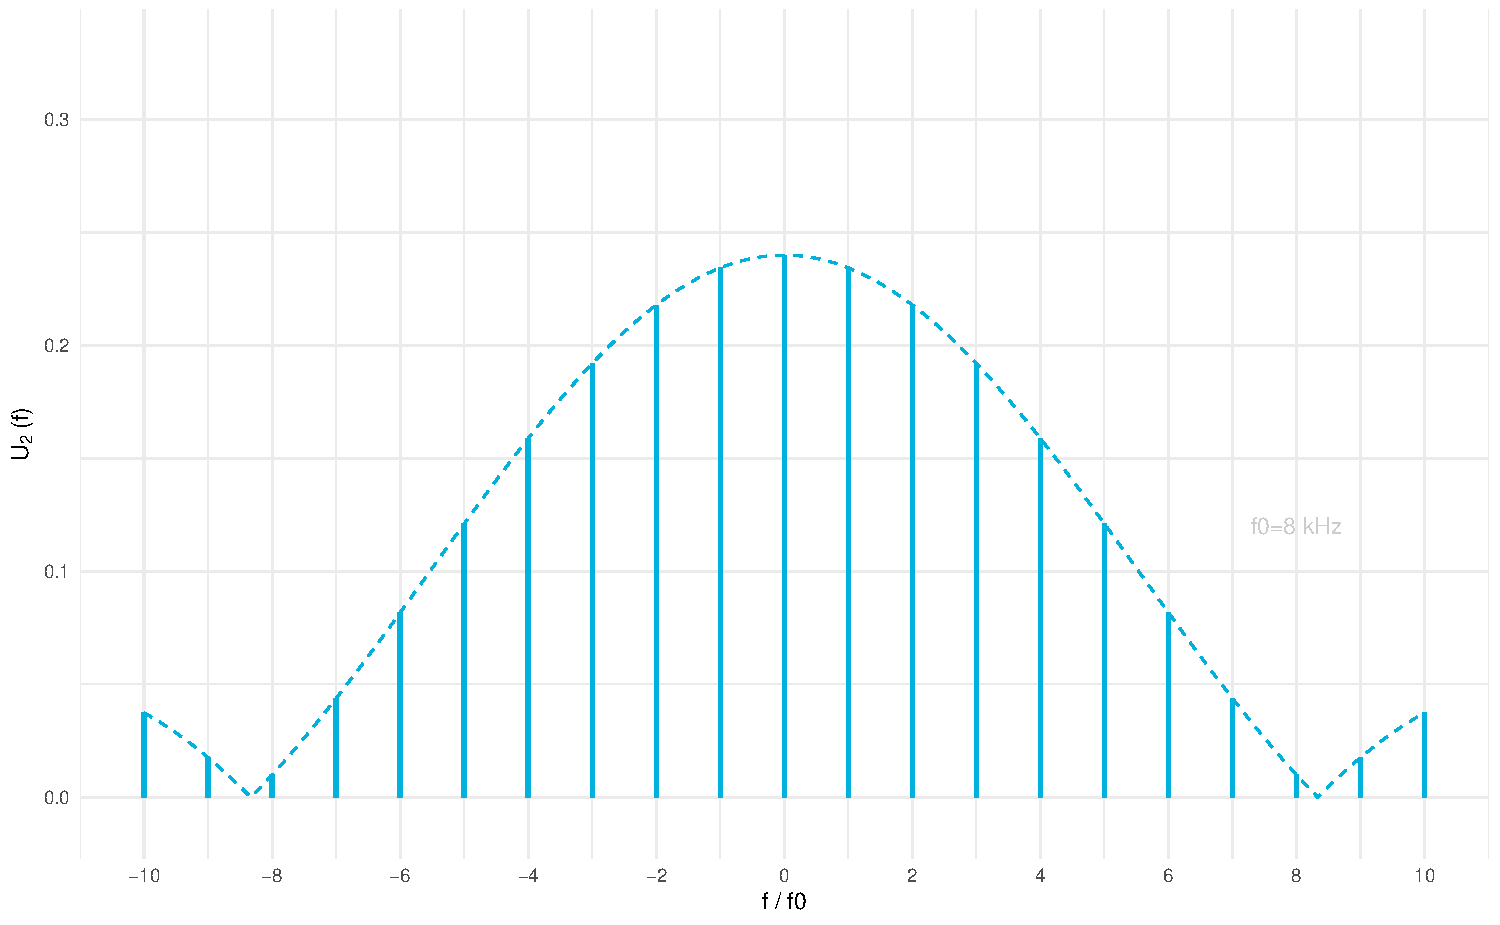
\includegraphics[width=\textwidth]{1_1/Si_8kHz}
  \caption{Teil des Spektrums der Rechteckimpulsfolge bei $T=1/8\,\si{\milli\second}$}
\end{figure}

Der Gleichanteil $a_0$ ist
\begin{gather*}
  \frac{a_0}{2} = \frac{1}{T} \cdot \int_{-T/2}^{T/2}{u_0(t) \dif t}\\
  = \frac{U_0}{T} \cdot \int_{-\tau/2}^{\tau/2}{ 1 \dif t} = \frac{U_0}{T} \cdot
  \left[ \frac{\tau}{2} - (- \frac{\tau}{2}) \right] 
\end{gather*}
\eqbox{a_0 = 2 \cdot  U_0 \cdot \frac{\tau}{T} }{0.618\textwidth}

\begin{figure}[H]
	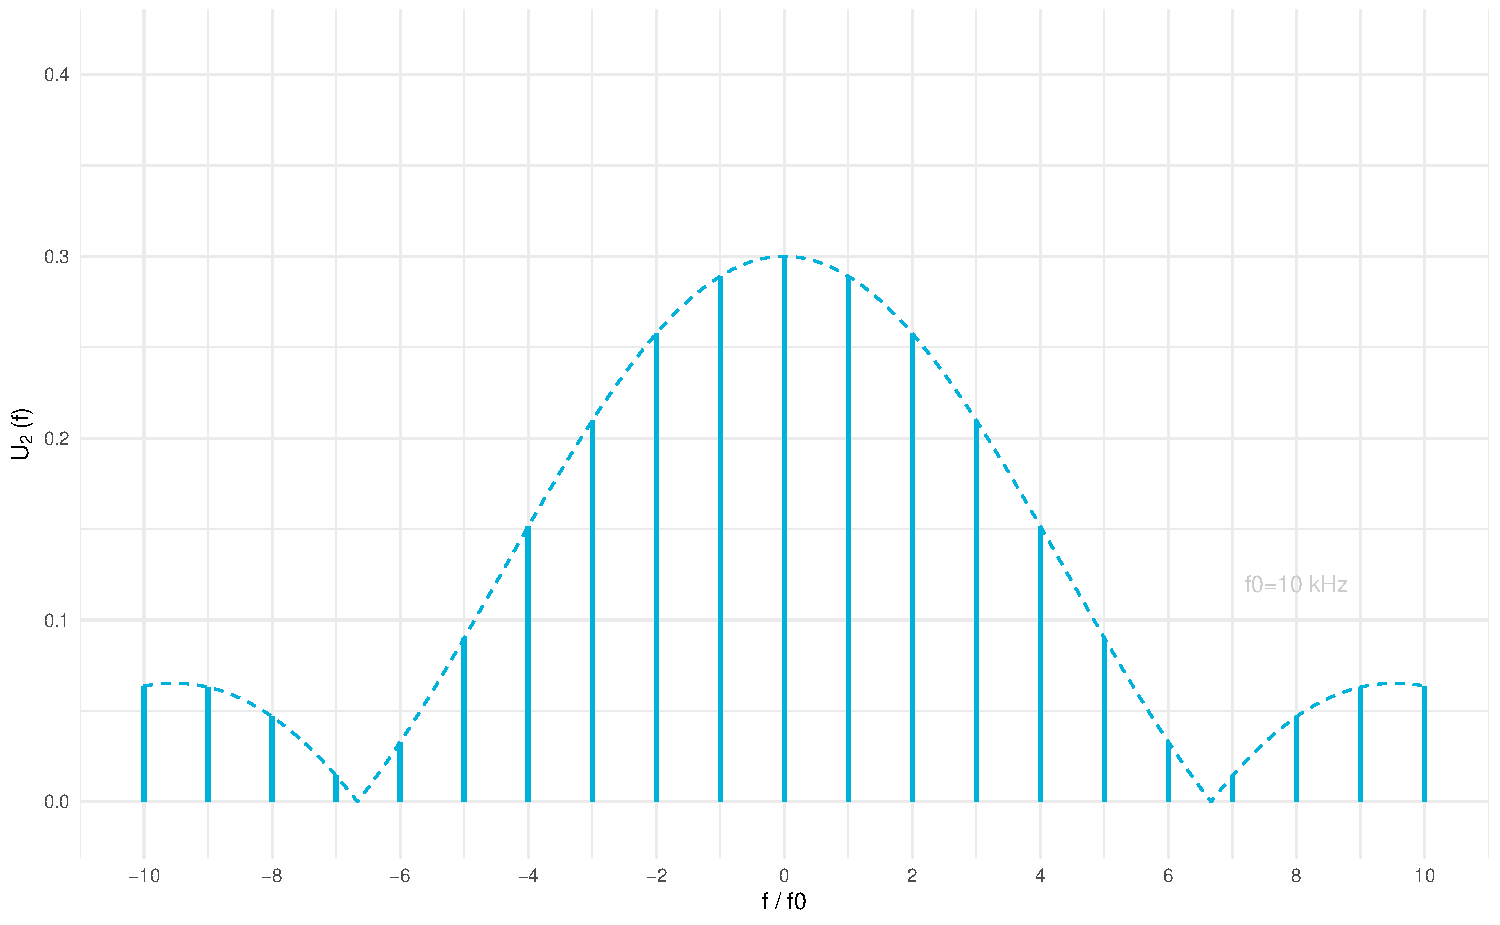
\includegraphics[width=\textwidth]{1_1/Si_10kHz}
  \caption{Teil des Spektrums der Rechteckimpulsfolge bei $T=1/10\,\si{\milli\second}$}
\end{figure}
%%%%%%%%%%%%%%%%%%%%%%%%
% 1.2

\subsection{}
Für die fehlerfreie Signalabtastung muss die Abtastfrequenz $f_A$ mindestens
doppelt so groß sein wie die maximal im Signal auftretende Frequenz $f_{SMax}$ (Nyquist-Theorem).
\[
  f_A \geq 2\cdot f_{SMax}
\]

Um die maximale Frequenz / die Bandbreite des Eingangssignals zu begrenzen muss
das Signal vor der Abtastung gefiltert werden.

%%%%%%%%%%%%%%%%%%%%%%%%
% 1.3

\subsection{}

Die Multiplikation des Eingangssignals $u_1(t)$ mit dem Diracimpulskamm $u_0(t)$
führt auf eine Faltung im Zeitbereich.
\[
U_2(f) = U_1(f) * U_0(f)
\]
Die Fouriertransformation des Dirac-Kammes $U_0(f)$
führt ebenfalls auf einen mit der Abtastperiode gedämpften Dirac-Kamm
\[
  u_0(t) \,\, \laplace \,\, \frac{1}{T_a} \cdot \sum_{k=-\infty}^{\infty}{\delta{(f - k
      \cdot \frac{1}{T_a})}}
\]

Die Faltung einer Funktion $f(x)$ mit einem Diracimpuls $\delta(x)$ führt zur Verschiebung dieser
Funktion an die Stelle des Diracs $B$ und Wichtung der Funktion mit dem Faktor $a$
\begin{equation}
\label{eq:1}
  f(x) * a \cdot \delta(x - B) = a \cdot f(x - B)
\end{equation}

Da ein Diracimpulskamm lediglich eine Summe mehrerer Diracimpulse ist, kann man
die Linearität des Faltungsintegrals ausnutzen
\begin{gather*}
  U_2(f) = U_1(f) * U_0(f)\\
  = \int_{-\infty}^{\infty}{U_1(F) \cdot U_0(F - f) \dif F}\\  
  = \frac{1}{T_a} \cdot \int{U_1(F) \cdot \sum_{k=-\infty}^{\infty}{\delta((F-f) - k
      \cdot \frac{1}{T_a})} \dif F }\\
  = \frac{1}{T_a} \cdot \left( \cdots + \underbrace{
      \int{U_1(F) \cdot \delta{(F-f)}}
    }_{\textrm{Gl. } (1)}
    +
    \underbrace{
      \int{U_1(F) \cdot \delta{((F-f) - \frac{1}{T_a})}}
      }_{\textrm{Gl. } (1)}
      + \cdots \right)
\end{gather*}

Es ergibt sich also die Summe der Faltungen der Funktion $U_1(f)$ mit den einzelnen
Diracimpulsen des Kammes, also im Falle des Frequenzbereiches die periodische Verschiebung
des Spektrums $U_1(f)$ um die Werte $k \cdot 1/T_a$ sowie die Skalierung mit
$1/T_a$.\\

(Das Spektrum des Eingangssignals $u_1(t) = U_0 \cdot \cos{(2 \pi \cdot
  f_1 \cdot t)}$ stellt zwei Spektrallinien bei $-f_1$ und $+f_1$ dar)

\begin{figure}[H]
	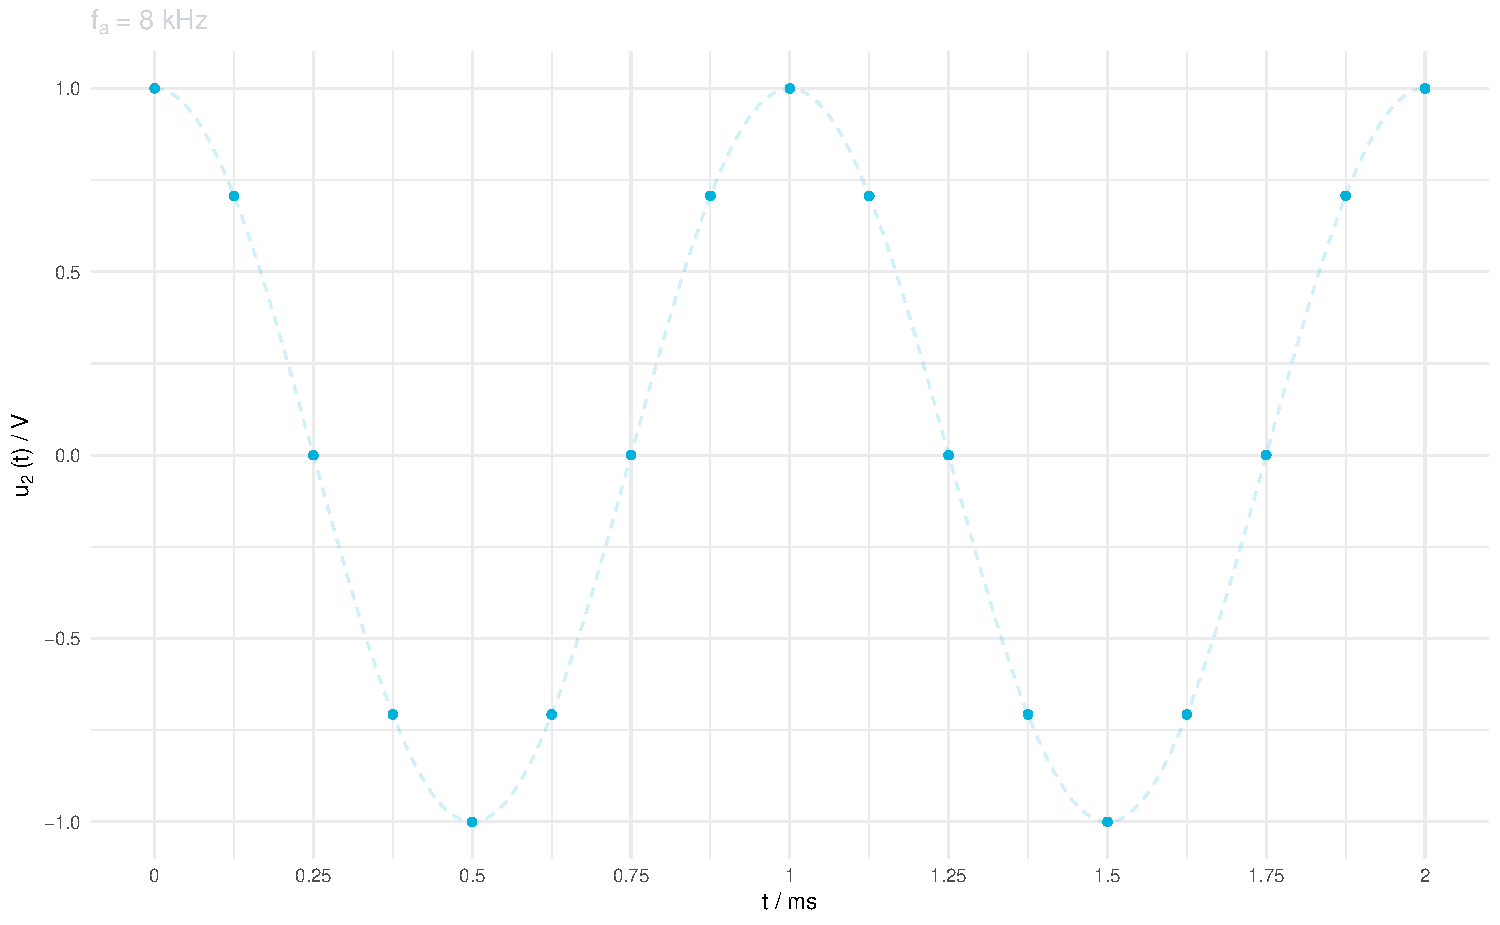
\includegraphics[width=\textwidth]{1_2/1_2_Abtast_8kHz_ZB}
  \caption{Zwei Perioden des Eingangssignals abgetastet mit $f_a=8\,\si{\kilo\hertz}$}
\end{figure}

\begin{figure}[H]
	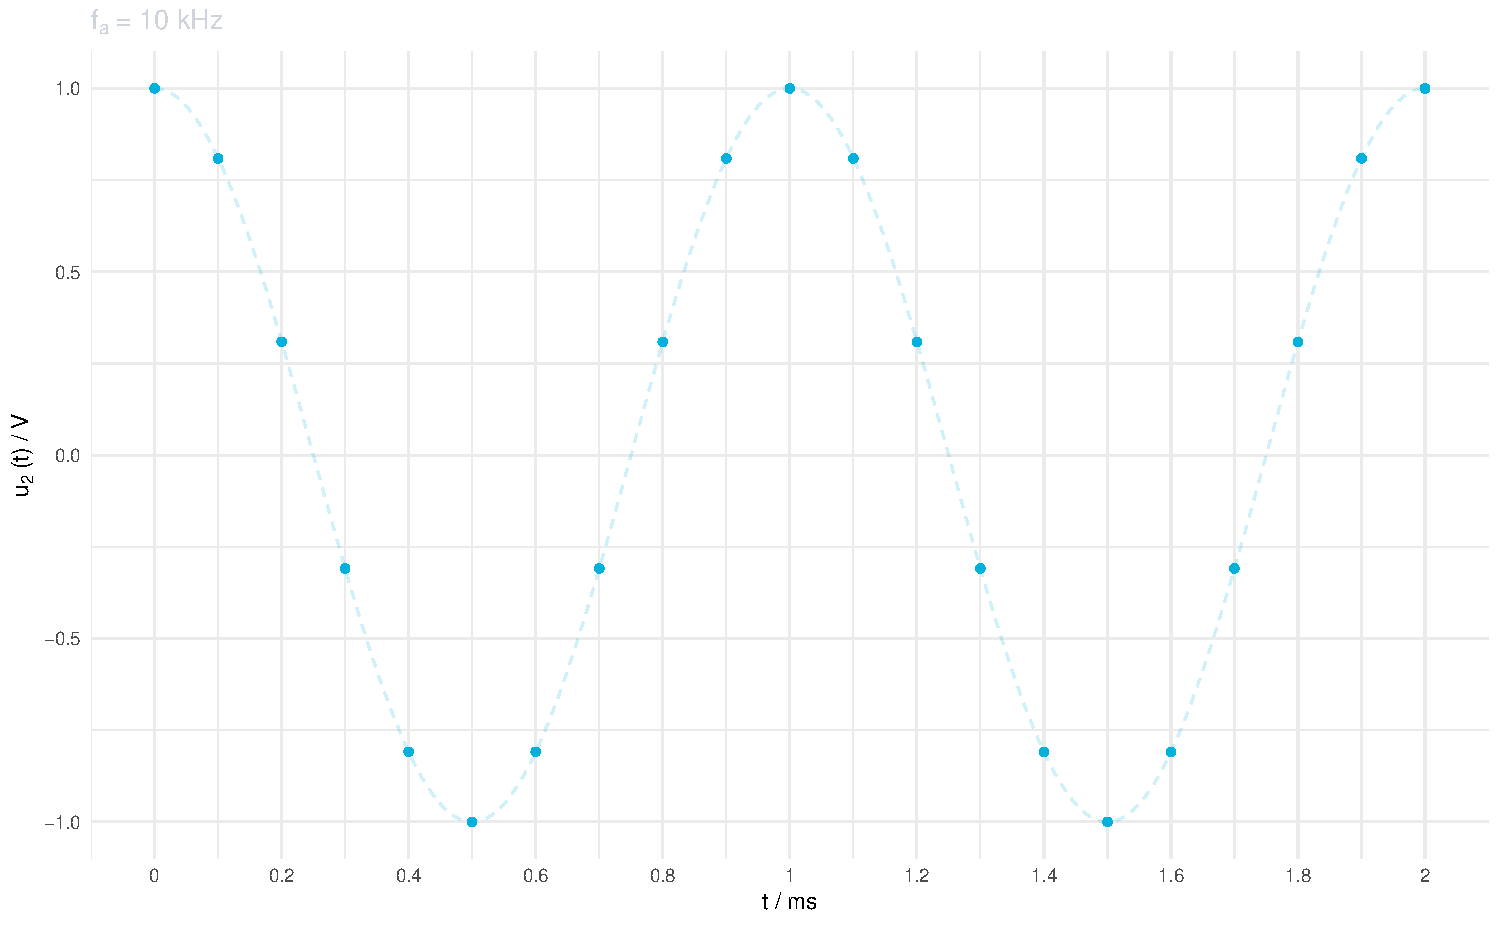
\includegraphics[width=\textwidth]{1_2/1_2_Abtast_10kHz_ZB}
  \caption{Zwei Perioden des Eingangssignals abgetastet mit $f_a=10\,\si{\kilo\hertz}$}
\end{figure}

\begin{figure}[H]
	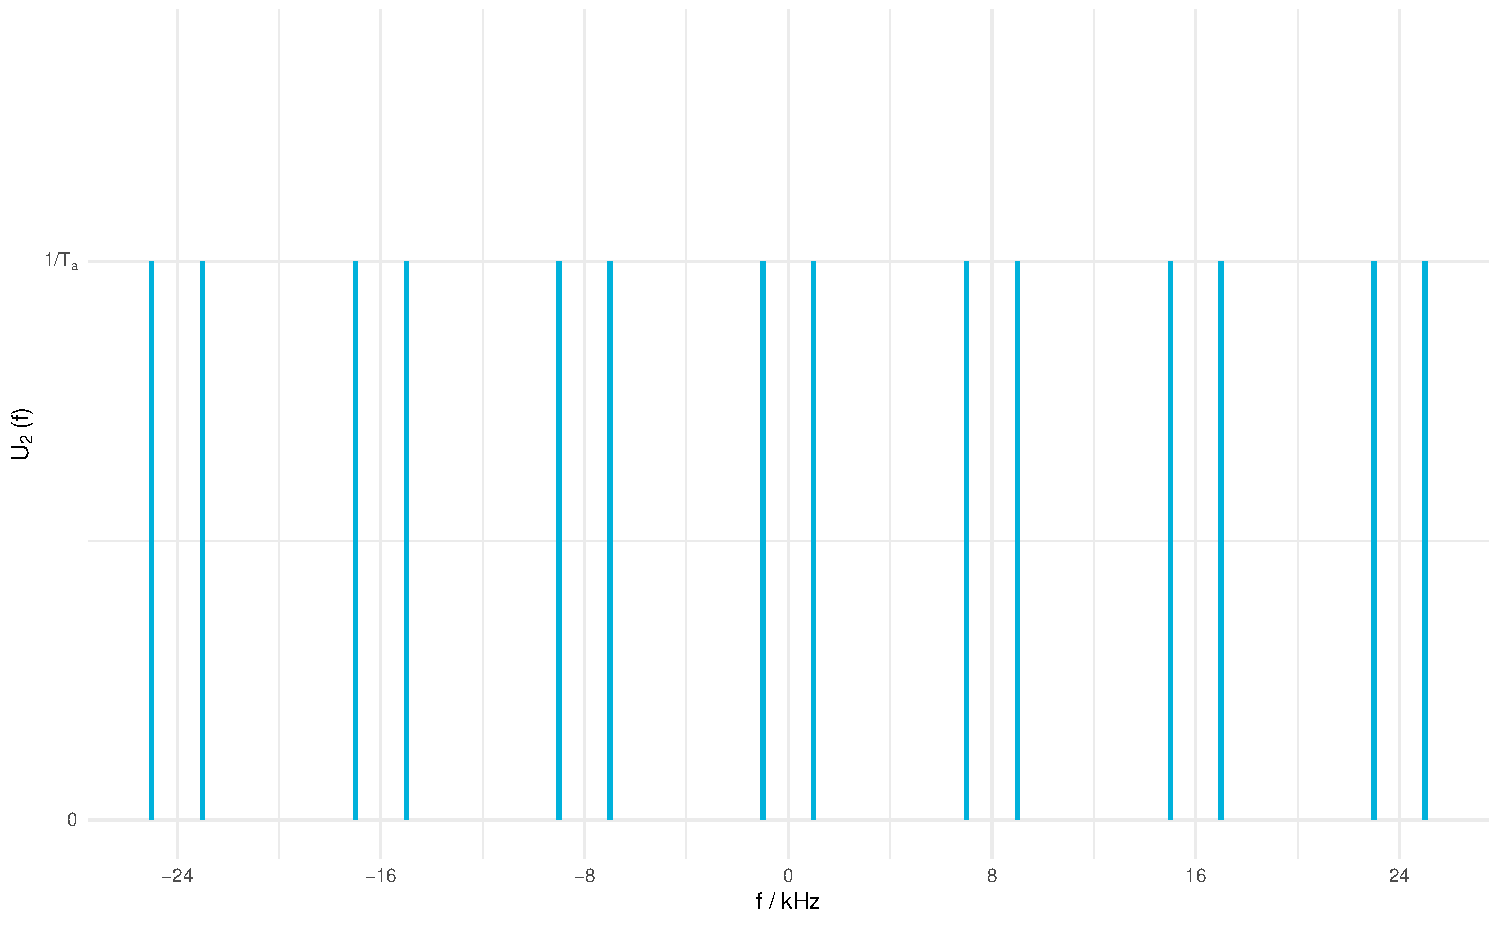
\includegraphics[width=\textwidth]{1_2/1_2_dirac_convolution_8kHz}
  \caption{Ausschnitt des Spektrums bei Abtastung mit $f_a = 8 \, \si{\kilo\hertz}$}
\end{figure}

\begin{figure}[H]
	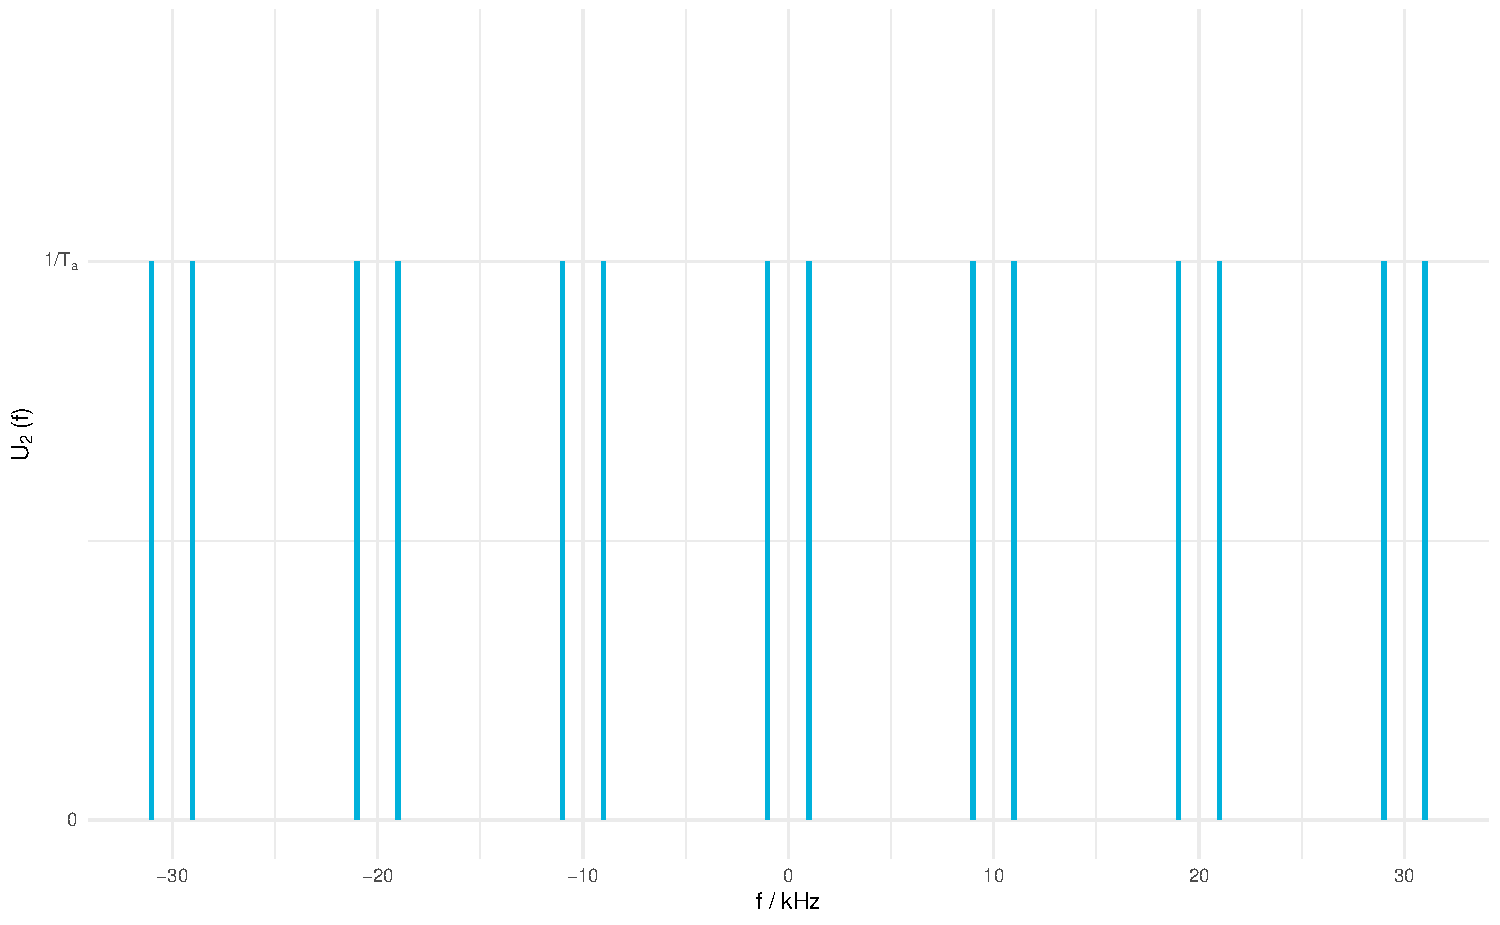
\includegraphics[width=\textwidth]{1_2/1_2_dirac_convolution_10kHz}
  \caption{Ausschnitt des Spektrums bei Abtastung mit $f_a = 10 \, \si{\kilo\hertz}$}
\end{figure}

Wird die Rechteckfolge aus 4.1. zur Abtastung verwendet, entsteht im Zeitbereich
eine stückweise kontinurierliche Funktion (Abb.).

Im Frequenzbereich entsteht die Faltung ähnlich wie bei der Abtastung mit dem
Dirackamm, nur dass das Spektrum mit dem gefaltet wird das diskrete Spektrum aus
Abb. 1 bzw. Abb. 2 ist.
Die Verschiebungen des Eingangssignalspektrums entstehen daher immernoch zu $k
\cdot 1/T_a$, die Wichtung der einzelnen Spektrallinien
ist jedoch nicht mehr konstant, sondern folgt der einhüllenden Si-Funktion des
Spektrums der Rechteckfolge.

\begin{figure}[H]
	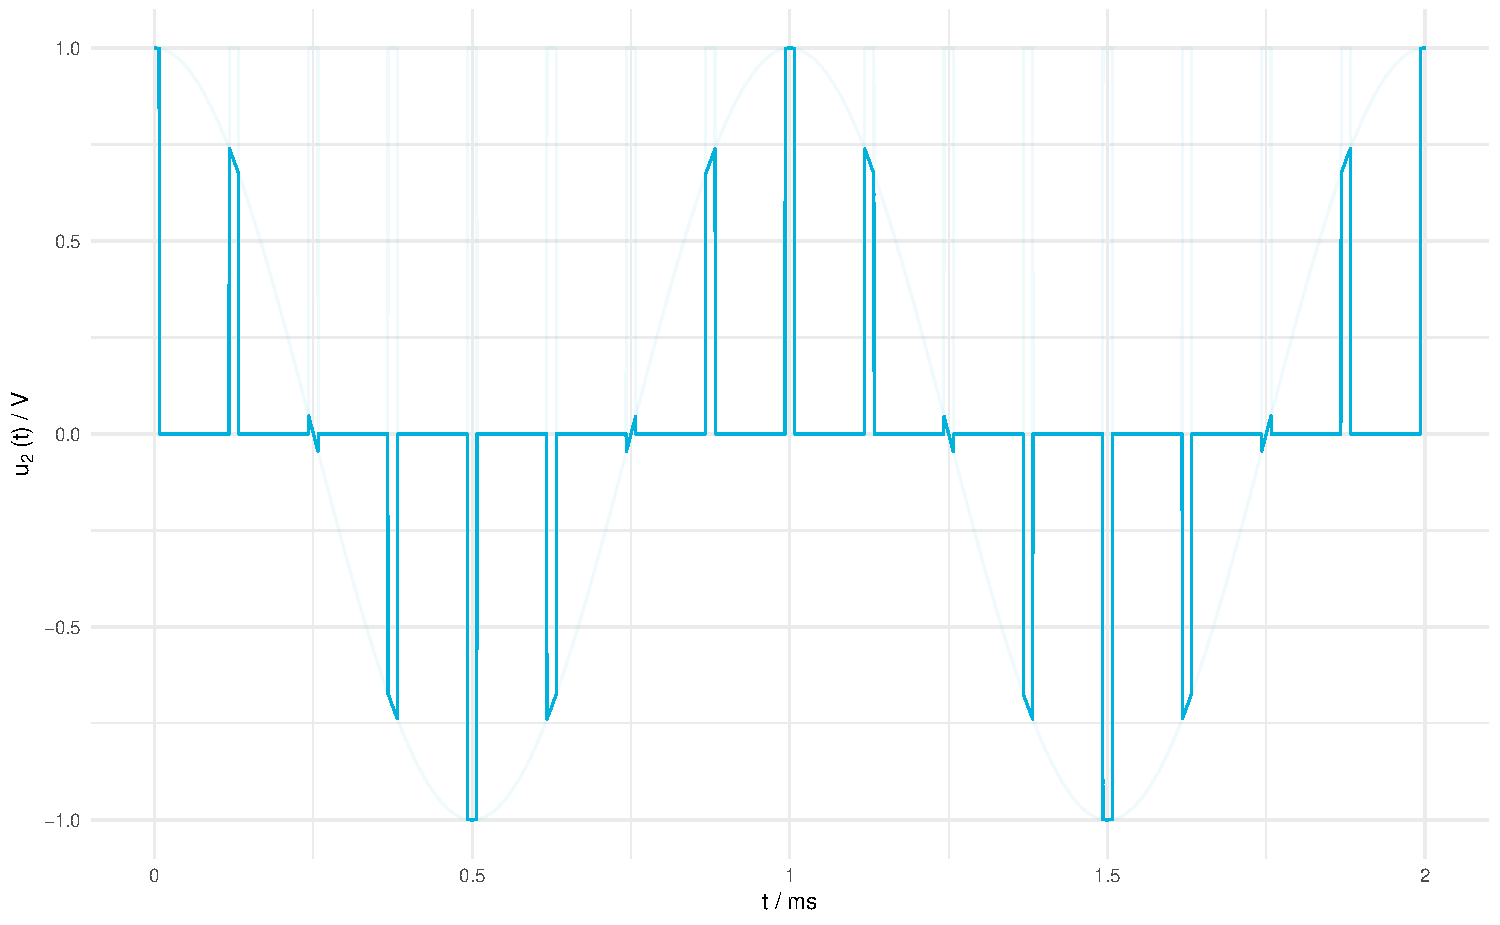
\includegraphics[width=\textwidth]{1_2/1_2_Abtast_Rechteck_ZB}
  \caption{Zwei Perioden des Eingangssignals abgetastet mit der periodischen
    Rechteckfolge aus 4.1 ($T=1/8 \,\si{\milli\second}$)}
\end{figure}

\begin{figure}[H]
	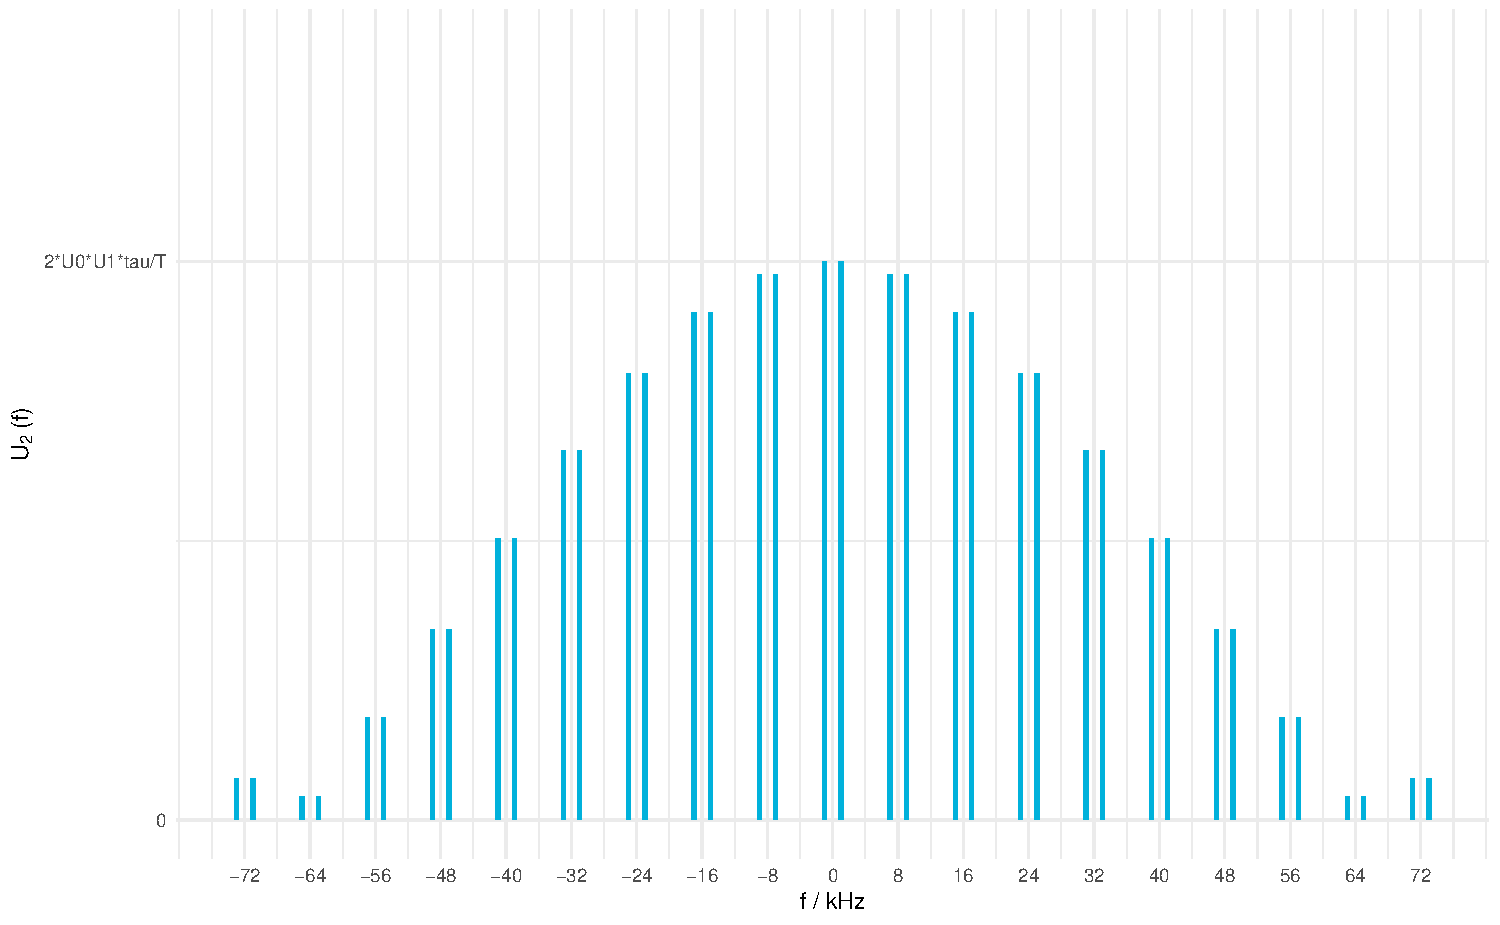
\includegraphics[width=\textwidth]{1_2/1_2_rechteck_convolution_8kHz}
  \caption{Teil des Spektrums bei Abtastung mit der Rechteckfolge aus 4.1 ($f_a = 8 \,\si{\kilo\hertz}$)}
\end{figure}


\section{Versuchsaufgaben}

\subsection{}
\begin{figure}[H]
	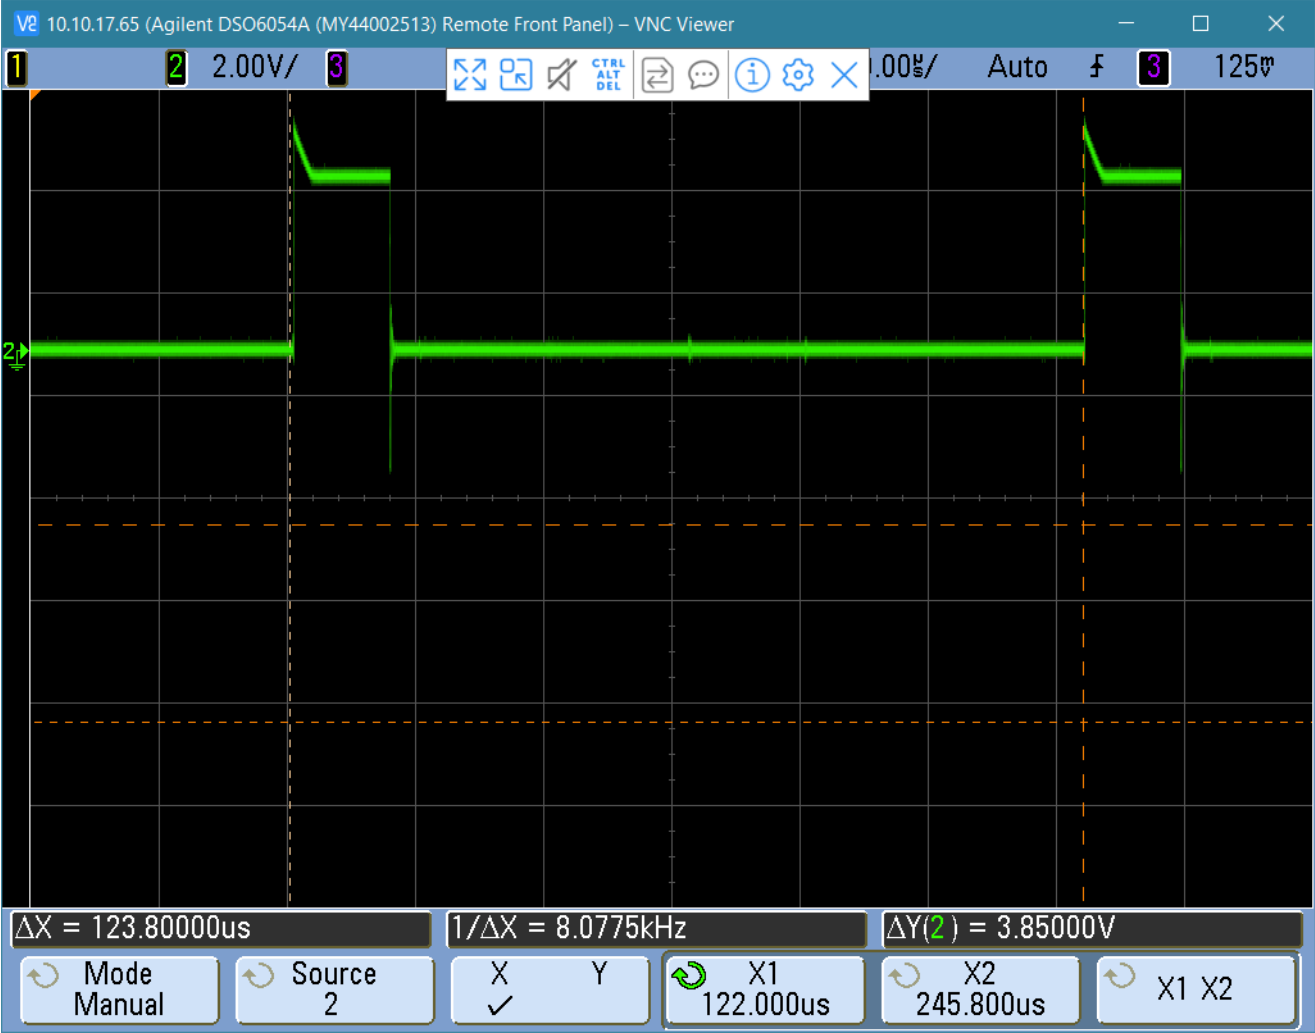
\includegraphics[width=\textwidth]{2_1/osz_abtast}
  \caption{Abtastsignal am Oszilloskop, Zeiteinstellung: $20 \, \si{\micro\second}/\textrm{div.}$}
\end{figure}

Aus der Oszilloskopmessung lässt sich eine Periodendauer von $T_a = 123 \, \si{\micro\second}$ und damit
eine Frequenz von $f_a = 8.0775 \, \si{\kilo\hertz}$ sowie eine
Impulsbreite von $\tau \approx 15.5 \, \si{\micro\second}$ ermitteln. Diese Werte
stimmen in etwa mit den Vorgaben der Vorbereitungsaufgaben überein. Da die
Impulsbreite leicht länger ist als die theoretische, ist eine Verschiebung der
Nullstelle der Einhüllenden Si-Funktion im Spektrum nach links zu erwarten.

\begin{figure}[H]
	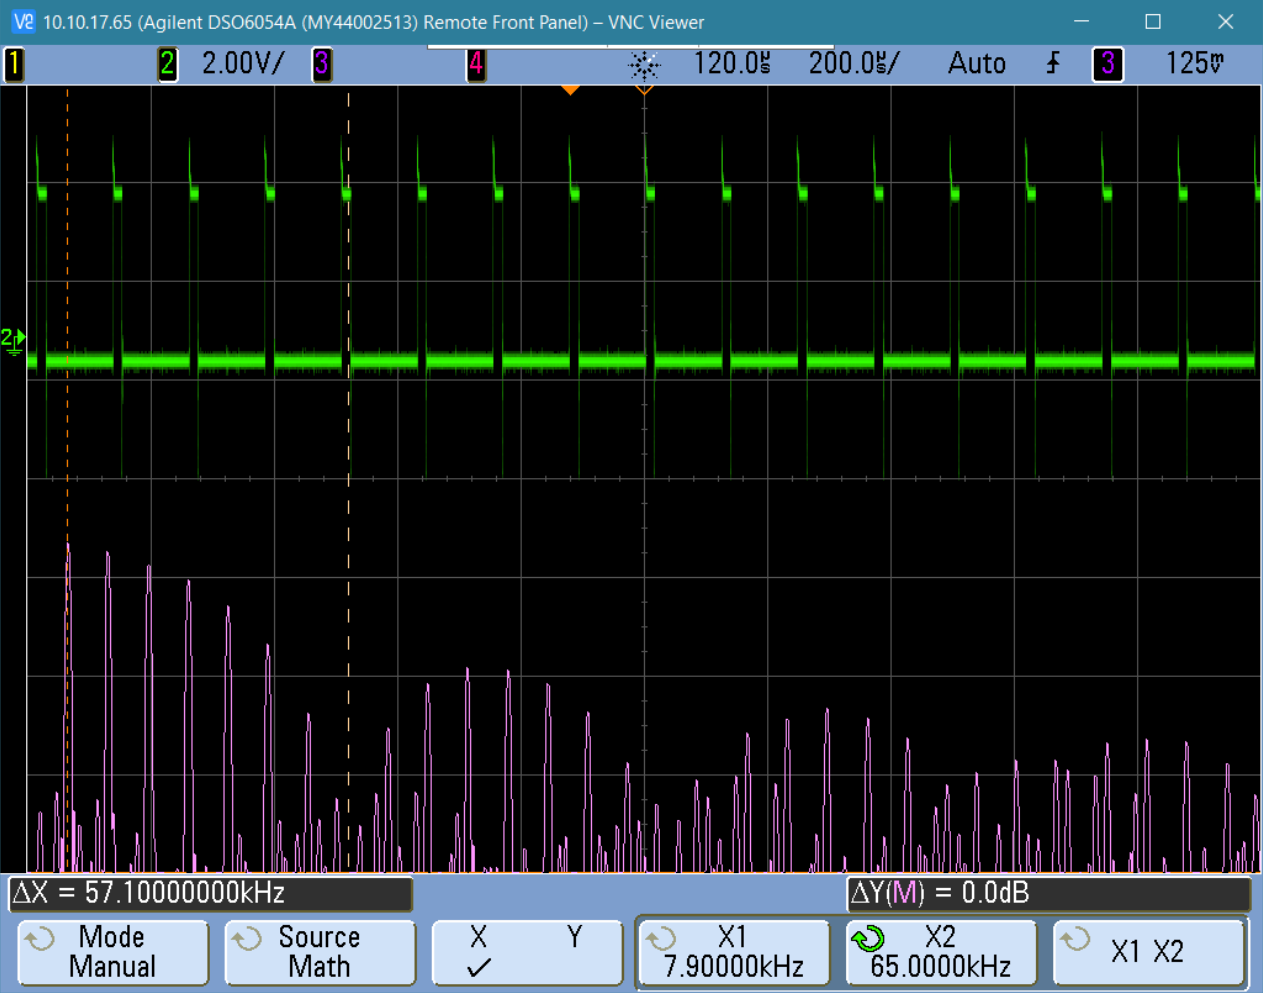
\includegraphics[width=\textwidth]{2_1/osz_abtast_fft}
  \caption{FFT des Abtastsignals}
\end{figure}

Der Frequenzabstand der Spektrallinien stimmt ebenfalls etwa mit dem
theoretischen ( $8 \, \si{\kilo\hertz}$ ) überein. Die theoretische Nullstelle
ist wie erwartet leicht verschoben.

\subsection{}
\begin{figure}[H]
	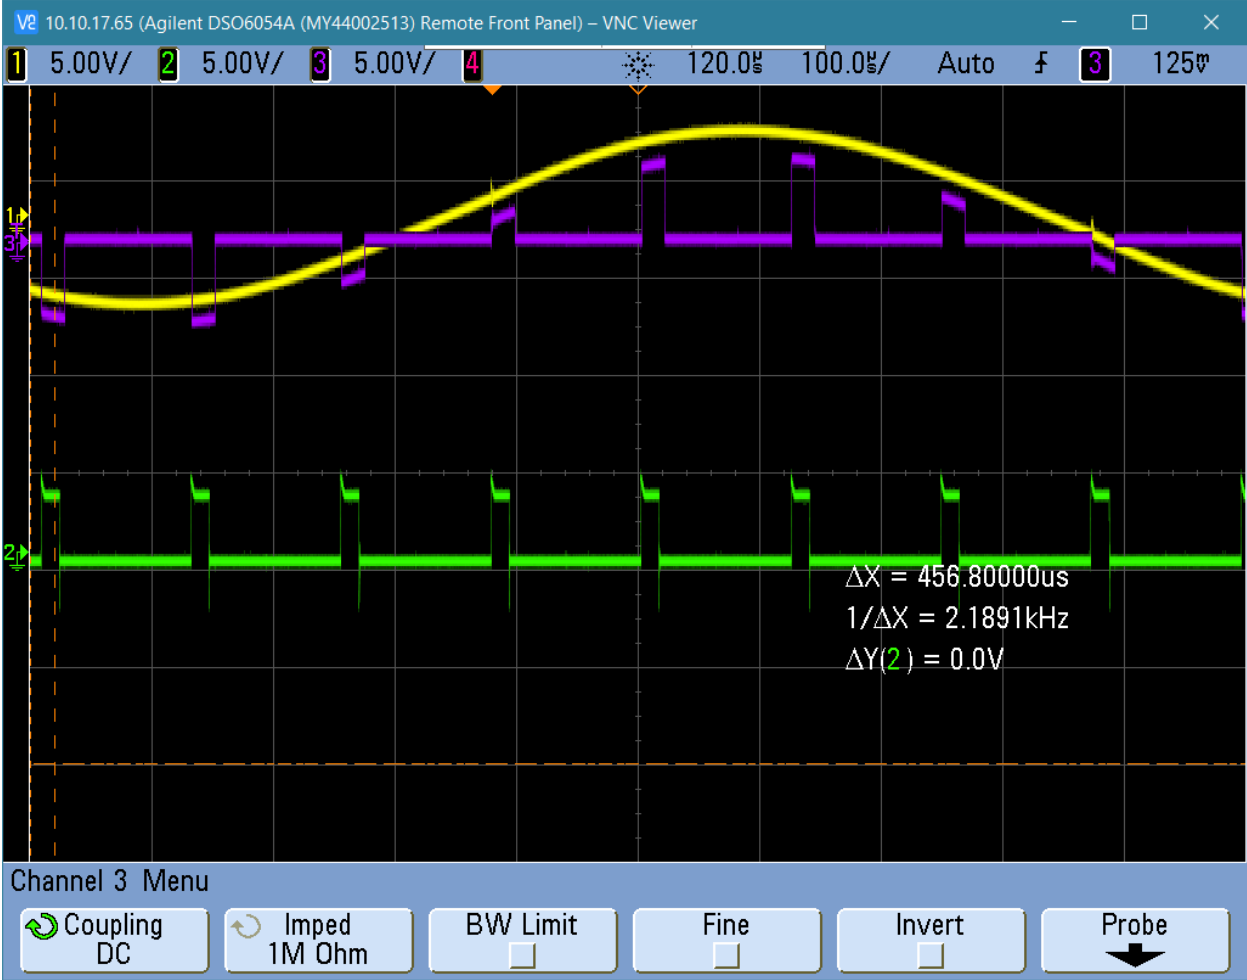
\includegraphics[width=\textwidth]{2_2/2_2_ZB}
  \caption{Abtastsignal (grün), Nachrichtensignal (gelb), und abgetastetes
    Signal (Violett) am Oszilloskop}
\end{figure}

Aus Abbildung 11 lässt sich die Multiplikation von Abtast- und Nachrichtensignal
erkennen. Bereits hier lässt sich eine zeitliche Verbreiterung der Impulse des
abgetasteten Signals gegenüber dem Abtastsignal erkennen. 


\begin{figure}[H]
	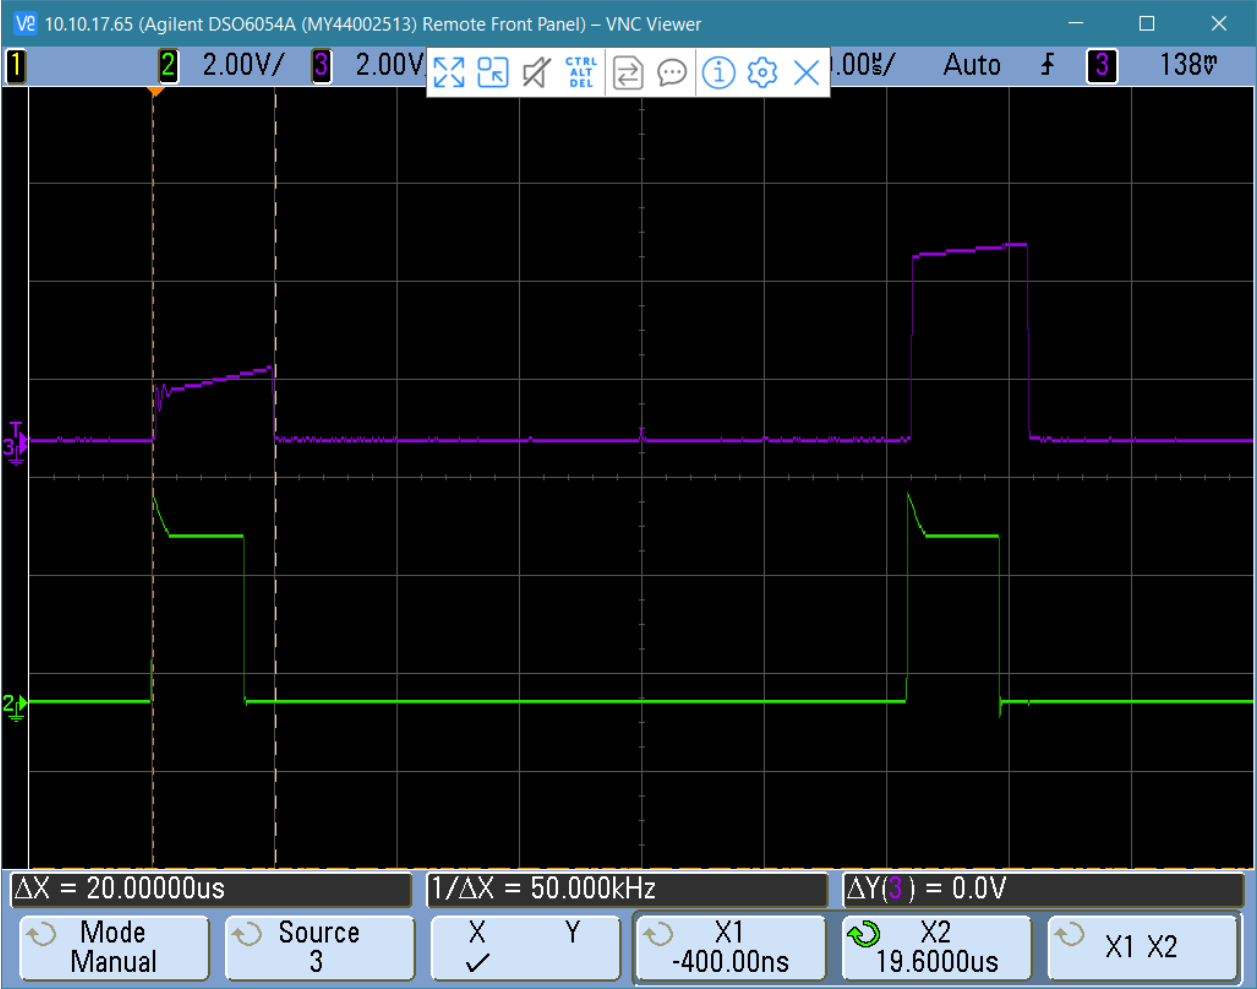
\includegraphics[width=\textwidth]{2_2/2_2_Impulsvergleich}
  \caption{Vergleich von Abtast- und Ausgangsimpulsen} 
\end{figure}

Bei genauerer Betrachtung erkennt man, dass die Impulsbreite des abgetasteten
Signals etwa $20 \, \si{\percent}$ größer ist als die der Abtastimpulsfolge.
Dies lässt sich auf die Trägheit des Systems zurückführen.

\begin{figure}[H]
	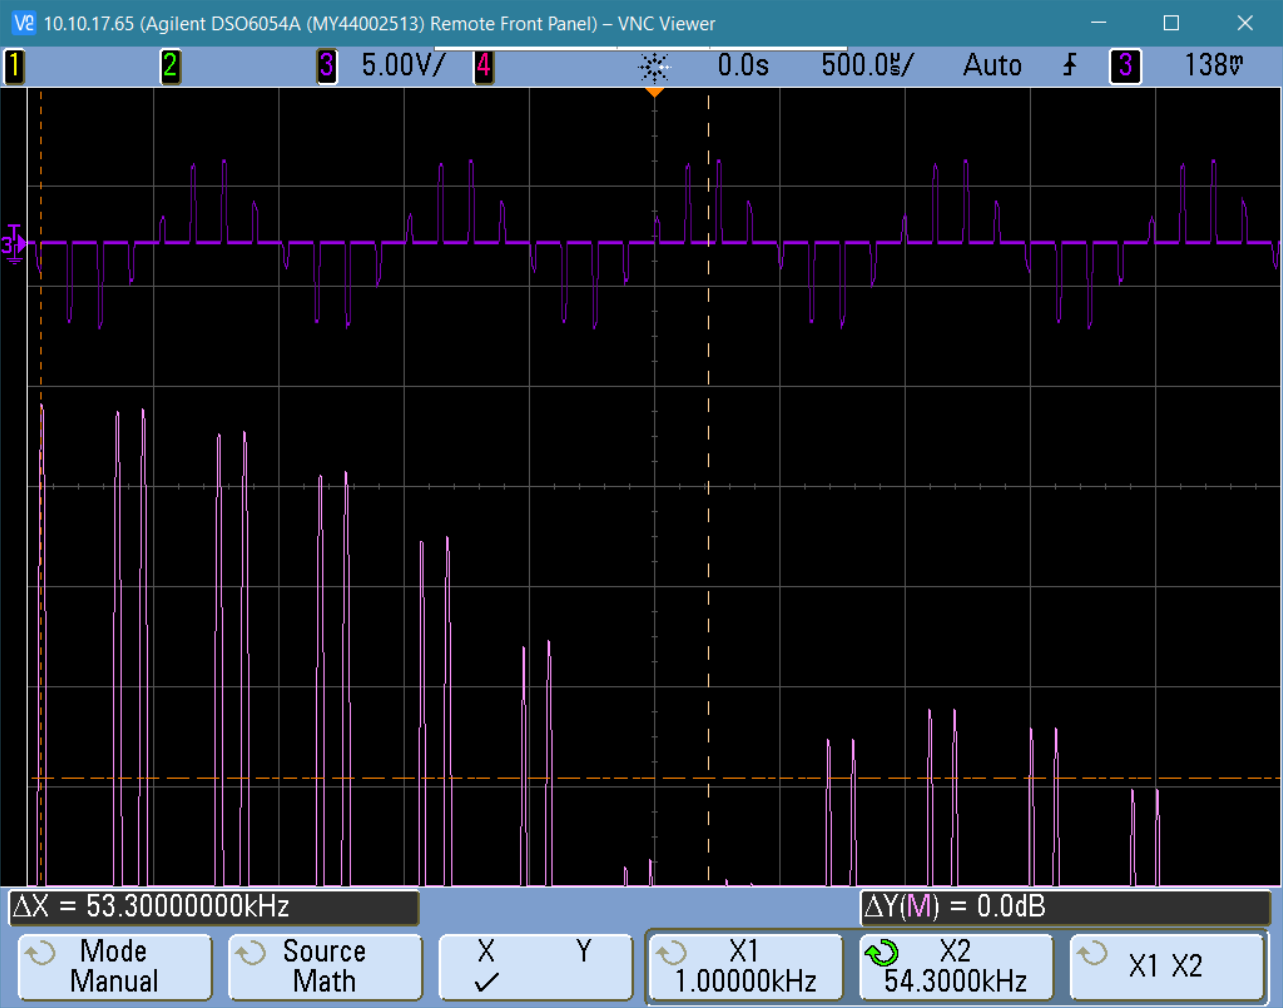
\includegraphics[width=\textwidth]{2_2/2_2_spektrum}
  \caption{FFT des PAM-Signals}
\end{figure}

Im Spektrum des Signals treten wie erwartet die Spektrallinien des Signals um
die Abtastfrequenz auf. 
Der Effekt der verringerten Impulsbreite spiegelt sich hier ebenfalls
wider, da sich die Nullstelle nun zu einer geringeren Frequenz bewegt (ebenfalls
ca. um $20 \, \si{\percent}$ verringert). 

\subsection{}
Die Quantisierungsstufenzahl $S$ errechnet sich bei einer Quantisierung mit $n$
Bits nach
\[ S = 2^n\]
Bei $6$ Bits ergeben sich also $2^6=64$ mögliche Stufen. Bei linearer
Quantisierung einer Spannung im Bereich $\pm 5 \, \si{\volt}$ erhält man einen
Stufenabstand $s$ von
\[ s = \frac{5 \, \si{\volt}}{32} =  156.25 \, \si{\milli\volt} \]
wenn man das MSB als Vorzeichenbit verwendet.

Durch Anlegen von Gleichspannungen und Ermittlung der Spannungswerte der
D/A-gewandelten Bitfolgen lässt sich die Quantisierungskennlinie darstellen

\begin{figure}[H]
	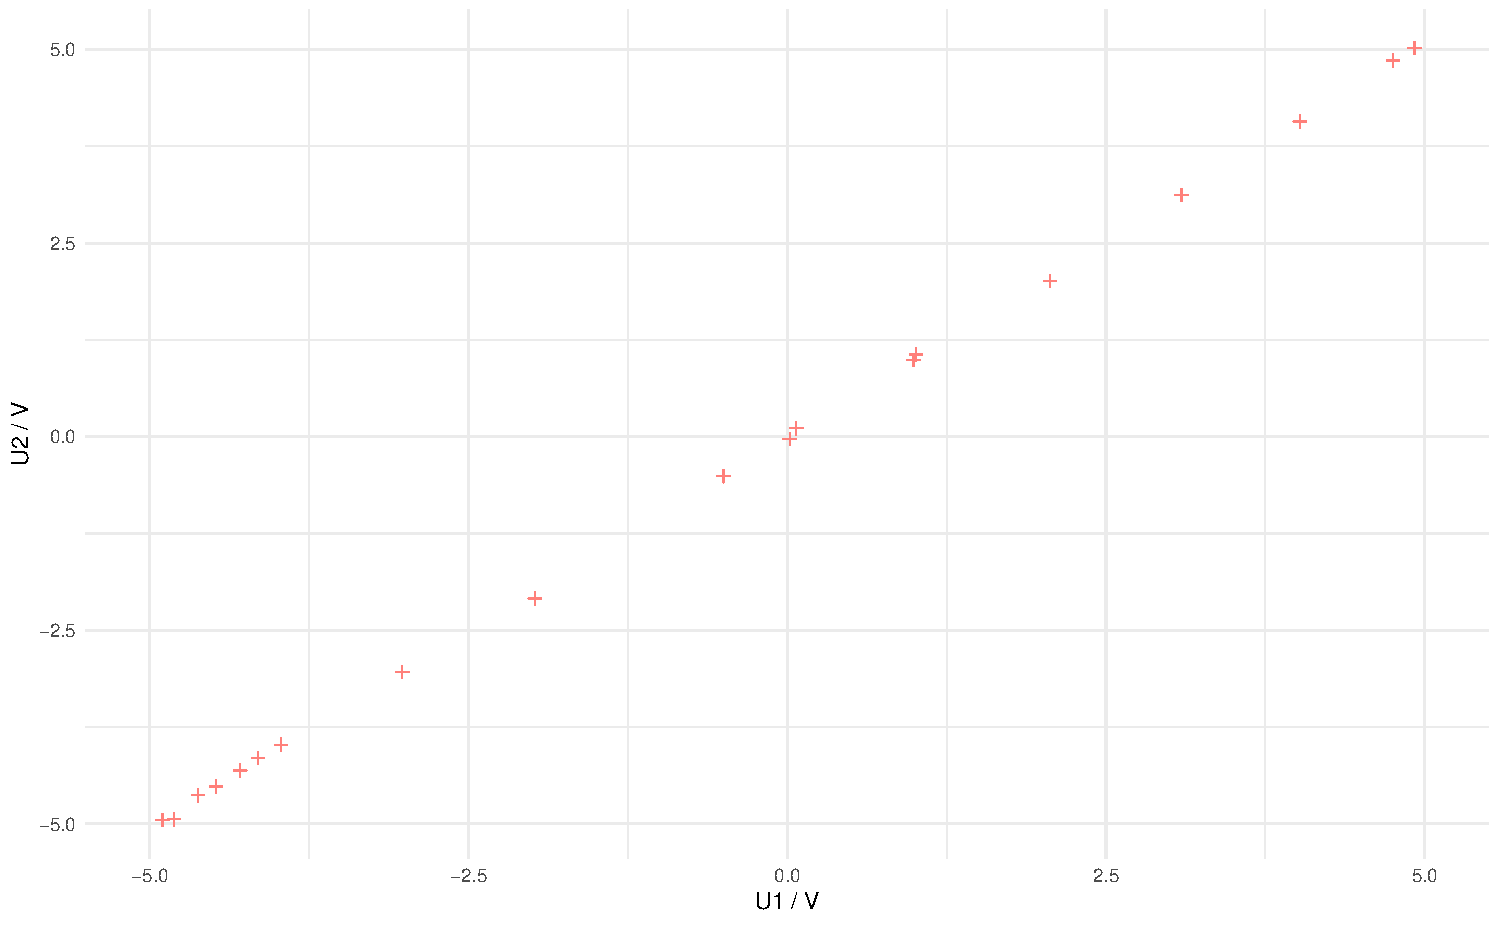
\includegraphics[width=\textwidth]{2_3/R/linquant_noc}
  \caption{Aufgenommene Werte der Ausgangsspannung über der Eingangsspannung}
\end{figure}

\begin{figure}[H]
	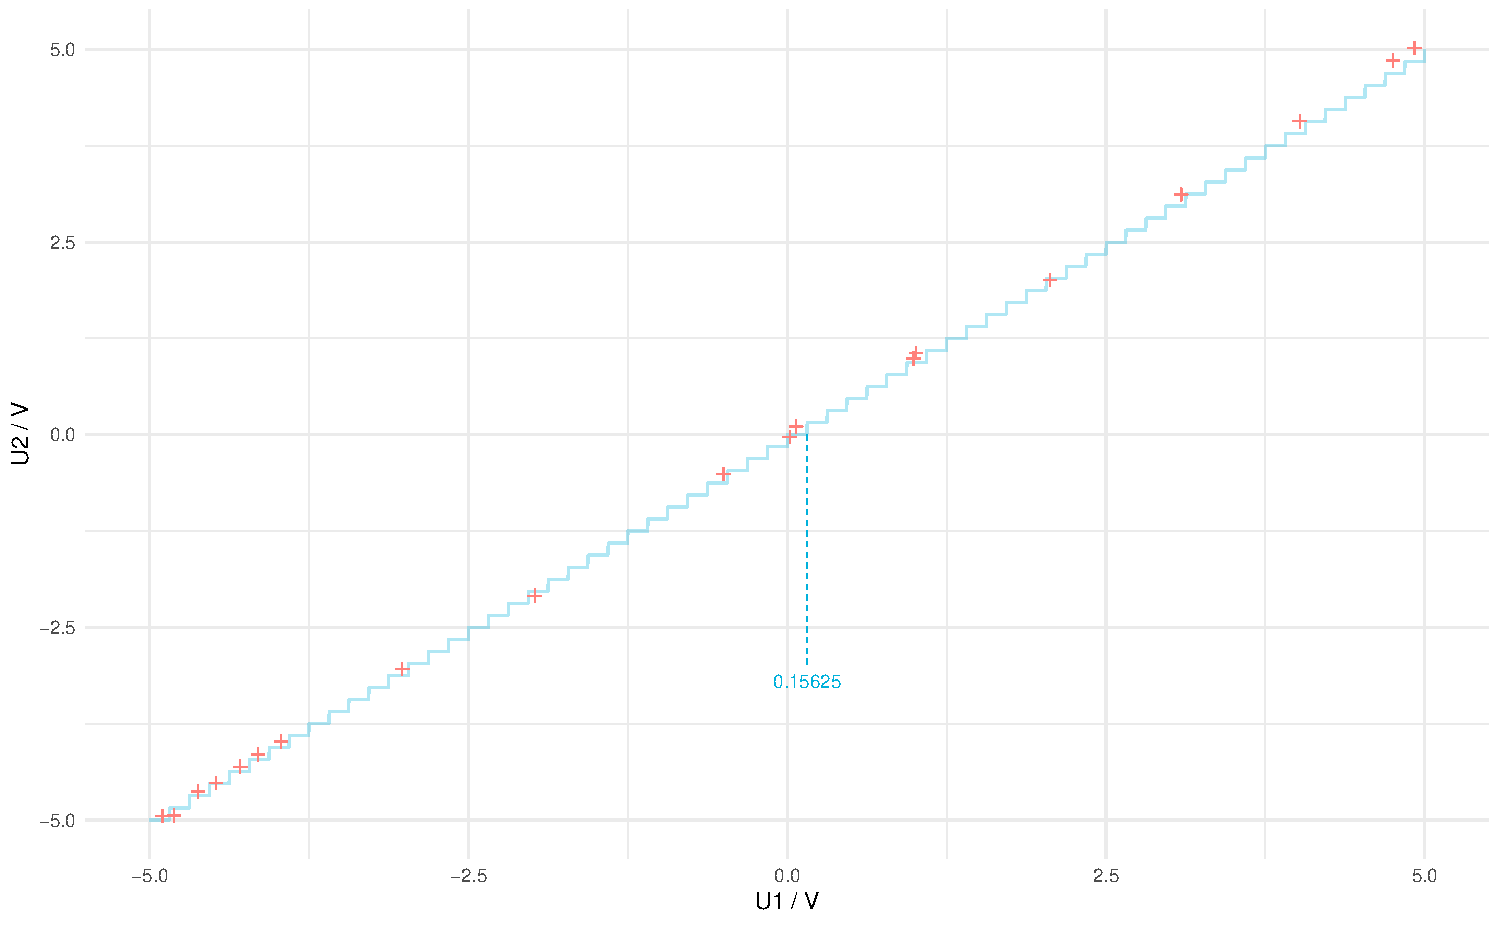
\includegraphics[width=\textwidth]{2_3/R/linquant_c}
  \caption{Aufgenommene Werte der Ausgangsspannung über der Eingangsspannung mit
  theoretischer Quantisierungskennlinie}
\end{figure}

\begin{figure}[H]
	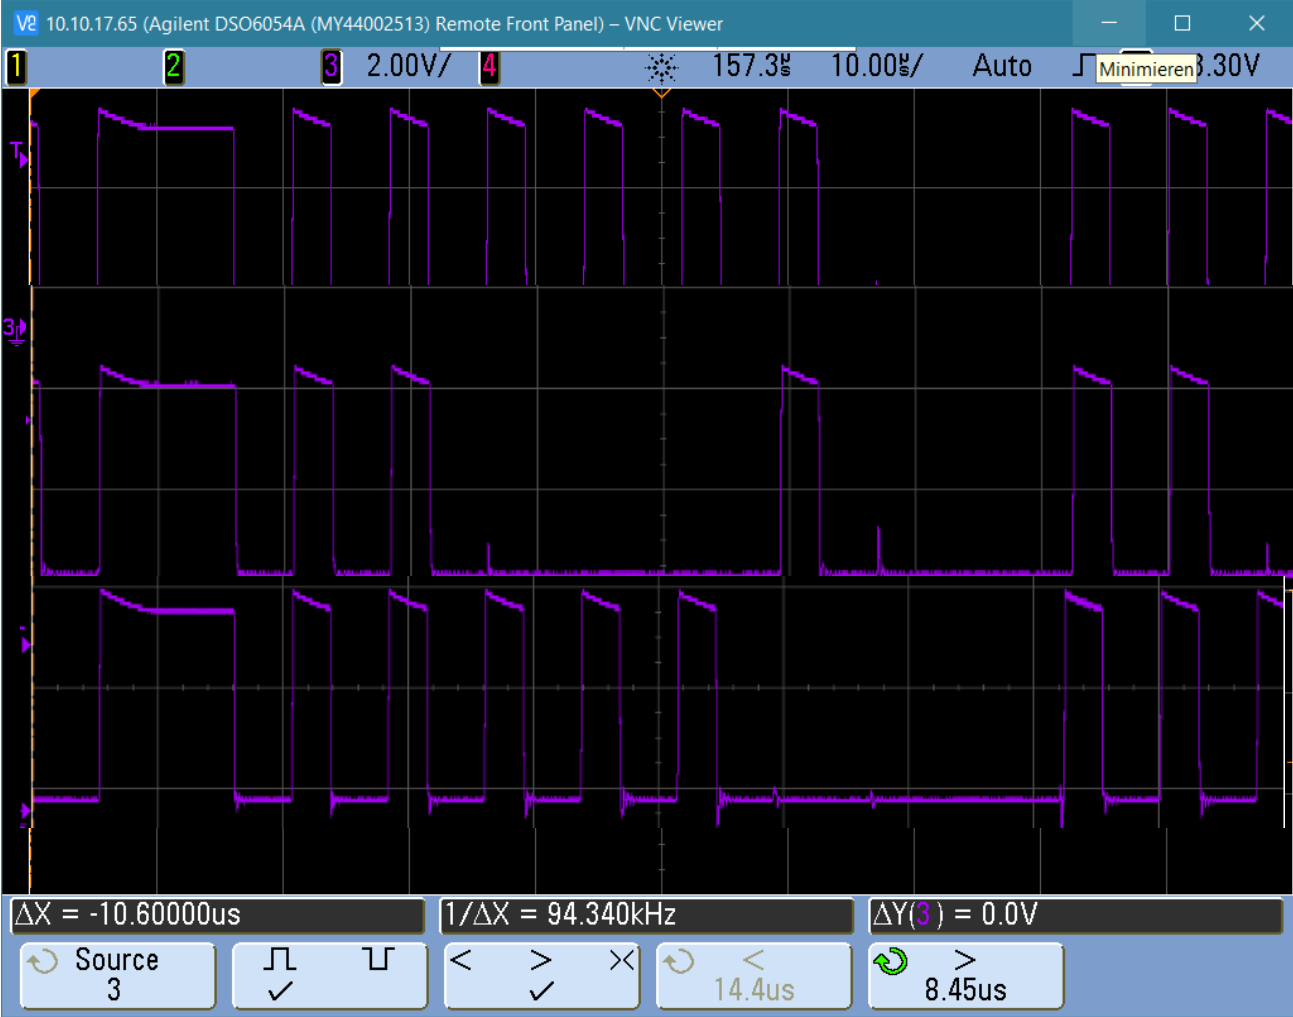
\includegraphics[width=\textwidth]{2_3/2_3_whatsmyvoltage}
  \caption{Darstellung einiger kodierter Spannungswerte nach der Quantisierung
    am Oszilloskop}
\end{figure}

Aus Abbildung 16 lassen sich die eingegangenen Spannungswerte über die
gemessenen Bitfolgen
ermitteln. Der etwas längere Synchronisierungsimpuls (links) bestimmt jeweils das Ende
der Bitfolge aus 2 Kanälen, je $6$ Bits.
Nimmt man an, dass das MSB bei einem HIGH-Pegel als positives, bei LOW-Pegel als
negatives Bit zu werten ist und dass der niedrigste Spannungswert
($-5\,\si{\volt}$) durch die Nullfolge (000000) dargstellt wird, ergeben sich
die folgenden eingangsseitigen Spannungswerte (als Intervall)

\begin{enumerate}
  \item[\textit{Oben:}]
    \begin{enumerate}
      Folge: 1 1 1 1 1 1\\
      Stufenwert: $(+)2^4+2^3+2^2+2^1+2^0=31$\\
      Spannungswert:  $31 \cdot s \, ... \, 32 \cdot s= +4.844 \,\si{\milli\volt}
      ... +5\,\si{\volt}$ 
    \end{enumerate}

  \item[\textit{Mitte:}]
    \begin{enumerate}
      Folge: 1 0 0 0 1 1\\
      Stufenwert: $(+)2^1+2^0 = 3$\\
      Spannungswert: $ 3 \cdot s ... 4 \cdot s = +468.75\,\si{\milli\volt}...+625\,\si{\milli\volt}$
    \end{enumerate}

  \item[\textit{Unten:}]
    \begin{enumerate}
      Folge: 0 1 1 1 1 1\\
      Stufenwert: $(-) 2^4+2^3+2^2+2^1+2^0 = (-)31$\\
      Spannungswert: $-1\cdot s ... 0 \cdot s = -156.25 \,\si{\milli\volt}...0
      \si{\volt}$ (000000 entspricht $-5 \,\si{\volt}$)
    \end{enumerate}

\end{enumerate}

%Bei der nichtlinearen Quantisierung ist die Stufung bei kleineren
%Spannungswerten feiner.
\end{document}
